\chapter{Feature Design for User Interaction in Spatially Augmented Reality Systems}

\fbox{This chapter is still in draft form}

In working with architects, I have gained keen insight into the needs of architects in the design process.  Ensuring that information is communicated clearly: both in relative dimensions and in terms of scale, ensuring intuitive interaction, maintaining interactive speed and properly introducing users to a system are all imperative in designing a system.  This section is a description of a few key features which could be added to our architectural daylighting system.  Both direct user feedback and our evaluation of details ignored by architects have shaped our design of the  following features.

\section{``Rendering Window'' on a small portable screen device}

\begin{figure*}[t]
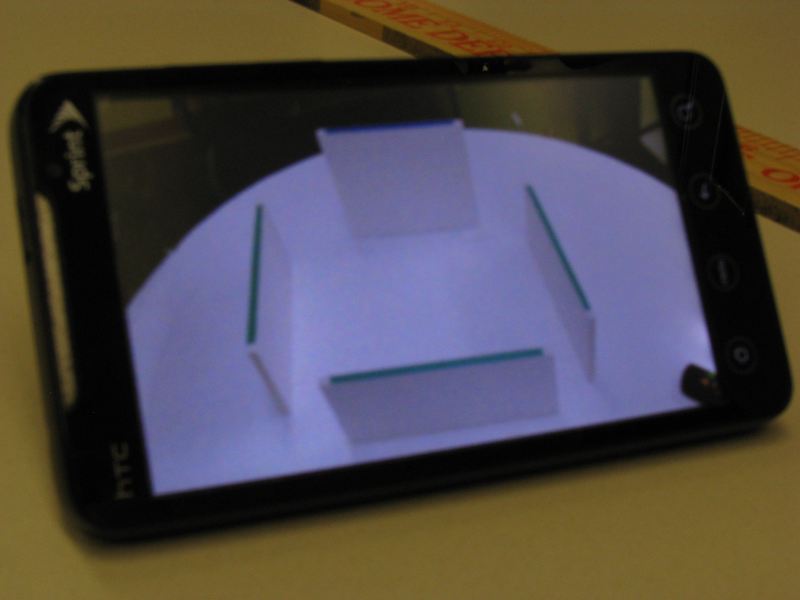
\includegraphics[width=0.31\textwidth]{images/IMG_1380.png}
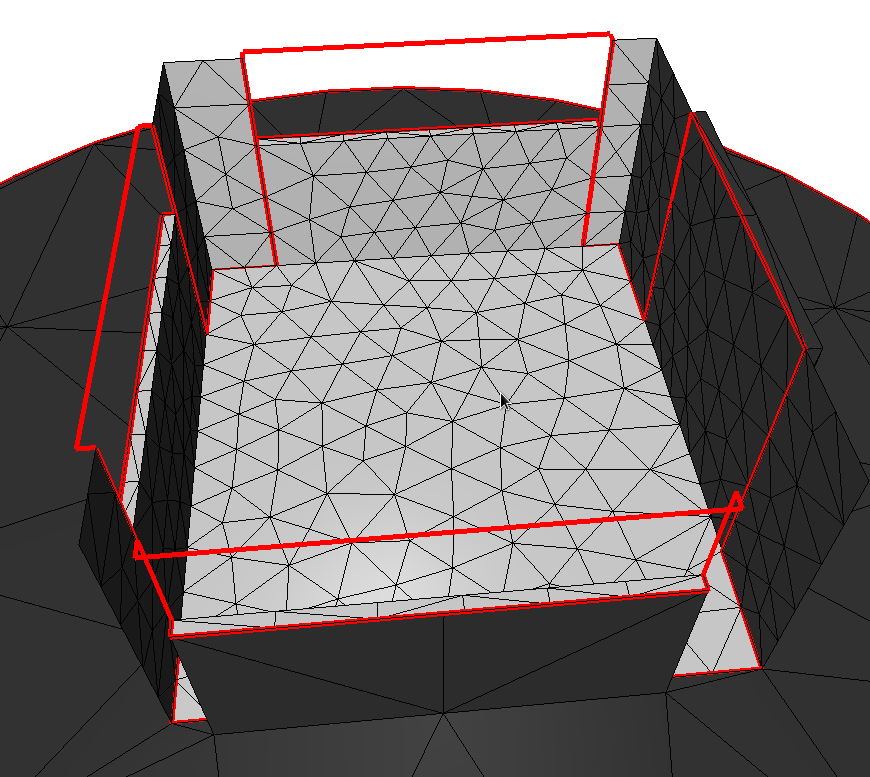
\includegraphics[width=0.31\textwidth]{images/remesher_screenshot.png}
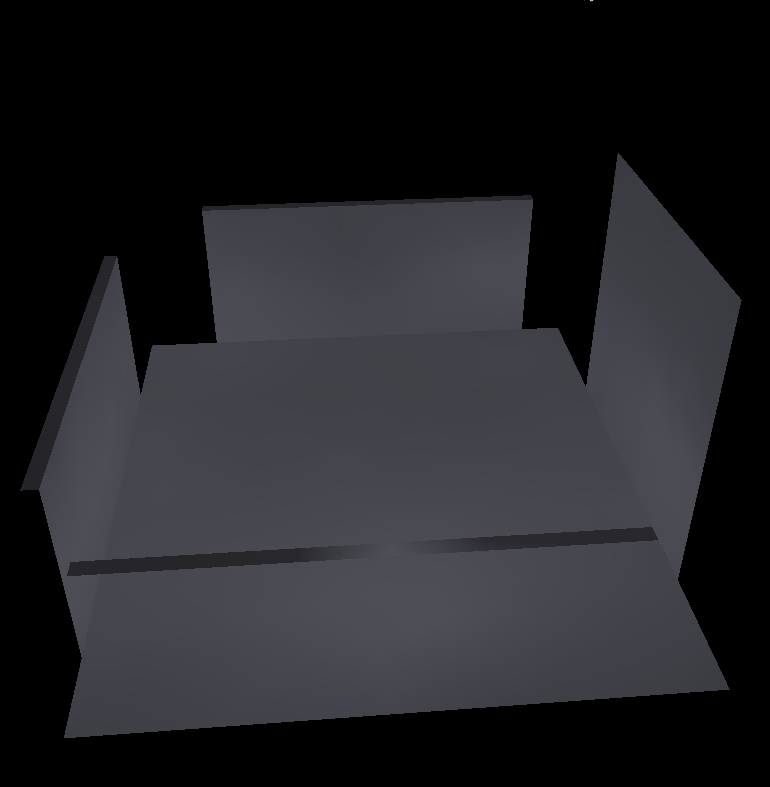
\includegraphics[width=0.31\textwidth]{images/lsv_screenshot.png}
\vspace{0.1in}\\
\begin{minipage}{0.31\textwidth}\vspace{-0.25in} \begin{center} Actual Image \end{center}\end{minipage}%
\begin{minipage}{0.31\textwidth}\vspace{-0.25in} \begin{center} Simulated Geometry \end{center}\end{minipage}%
\begin{minipage}{0.31\textwidth}\vspace{-0.25in} \begin{center} Simulated Daylighting \end{center}\end{minipage}%
\vspace{-0.25in}

\caption{Example Screenshots for Lighting Window Viewer}
\end{figure*}

In working with a 1/12 scale tangible projection interface, one of the largest limitations is that of resolution.  The resolution of the projectors around the tabletop are 1024 by 768.  Unfortunately, this resolution is not consistently achieved on the tabletop because the projectors are not at traditional angles to the projection surface.  While sufficient resolution to understand general lighting principles is achieved, additional visualizations are limited by this factor.  

While lighting is displayed clearly on the surfaces, information about geometry that does not have a physical representation cannot effectively be communicated to the user through the existing interface.  Some users expressed interest in having auto-generated furniture in the space.  Our collaborators have need of invisible sensor planes (such as a plane at the height of desk surfaces) to understand what the lighting levels will be like in an office space at working height.  

I propose an alternate way of viewing the scene while still using the physical table top for design.  By using a mobile device which contains a camera and LCD screen, a device could be situated in such a way that it acts as a window into the 3-dimensional scene as initially presented by Ishii and Ullmer\cite{Ishii97tangiblebits}.  As an example device, we could use a mobile smart phone such as the HTC EVO or the Apple iPhone as seen in figure 4.1.  The integral parts of these devices would be a camera, a wifi interface and a medium resolution display (at least 480p).  The camera would be used to take a picture of the scene from a location high enough that all the wall tops are visible.  This image would then be sent back to a machine for processing.  Computer vision detection techniques would then be used to ascertain the viewpoint from the camera based on the configuration of wall tops.  A unique configuration should be able to be discovered in most non-symmetric situations.  Situations in which all the wall tops are not visible present a difficult problem, but given that it is a reasonable assumption that the device be physically above all of the wall tops, it is a reasonable assumption that all wall tops be in view.  Once the wall positions are found these coordinates would have to be converted into model space coordinates so that a GLCamera could be found for the position in relation to room.  Once this is found this could be passed into Light Solve Viewer so that this perspective could be rendered.

The research problem solved would be creating a unique interface to interact with the space.  The computer vision involved would be the problem of given a known geometry, determining what perspective the camera is taking the picture from.  We are not attempting to determine the full 3-D geometry from this camera; we are assuming that the geometry will already be known from the existing system.  A good starting point for this problem would be choosing a number of viewpoints.  These viewpoints could be assumed to be 1.5 and 2.5 feet above the table plane from 10 equally spaced points around the circumference of the table.  Some example viewpoints are shown in figure 4.2.  It should be possible to simply look at the primitives seen (simply the colored parts on top) and see which viewpoint is most similar.  Once this works this could be extended to more viewpoints. 

One problem which we will be forced to solve is that in the current configuration all walls of the same height are the same color on the top with no distinguishing characteristics.  This would make solving for the position of walls in relation to one another a very difficult problem in certain cases.  Constraints will initially have to be made on the system to simplify this problem.  Early test cases could have one wall of a different color (and height) from the rest.  This will enable an algorithm to have a starting point when evaluating how well a wall configuration fits with the known scene.

An input device would also be necessary to show where these desk, tables, etc. would be positioned but given this information, this `window' would allow additional objects to be seen (along with their appropriate daylighting) without creating primitives for all of them.  This should not affect the spirit of the system as the system still will be using rooms designed using 3-dimensional primitives. \\


\begin{figure*}[t]
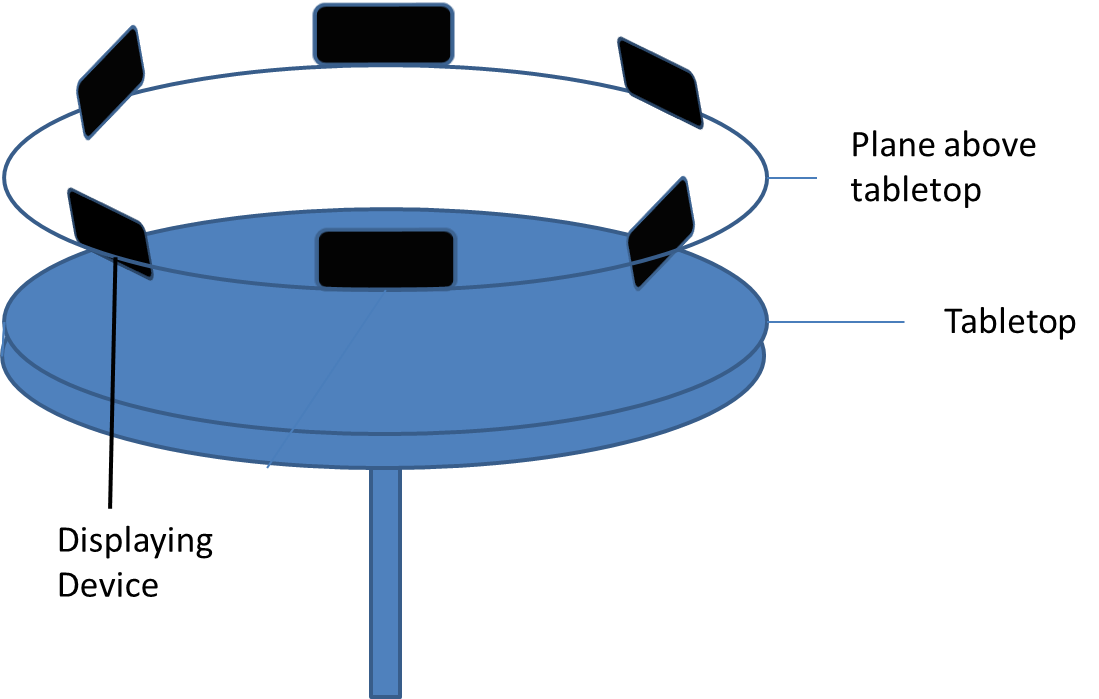
\includegraphics[width=.75\textwidth]{images/example_display_layout.png}
\caption[Example prototype of the daylighting window]{An early prototype of the daylighting window: the closest of a fixed number of viewpoints could be displayed.  These are example viewpoints.}

\end{figure*}

\section{Token specifying viewpoint added to the tabletop system}
\label{token}
Because Contraption has been using a radiosity solution to compute lighting, there have been some very specific limitations to the system.  The first limitation is that it was necessary to use a diffuse material model.  Radiosity assumes that all materials are lambertian, light is reflected in all directions with equal probability.  In standard offices, this assumption as often close to correct; however, in spaces with stylistic lighting, or even spaces that contain mirrors or many metallic objects this assumption falls apart very quickly.  Photon mapping allows specular and other non-diffuse materials because the material model can be programmed into the algorithm.  This property allows us to add functionality to the renderer to do glare calculations better.

Glare is defined as difficulty seeing in the presence of a bright light.  Glare is directly affected by the direction of a viewer in a space.  As such, I  propose adding a token to the tabletop system which indicates both the x and y position of a user in the space (with the height being assumed to be someone of average height) as well as the direction of the viewer.  The vision code running contraption will be slightly extended to properly detect this new token and from that glare can be calculated.  Please read on to the next two extensions for how I plan to display this information.  

\section{False color renderings for areas that are too bright, too dark, or contain glare}

Architects using the contraption system commonly noticed areas that were comparatively bright or dark in the scene, but they often did not have a good sense of what `too bright' or `too dark' were.  This could be due in part to the fact that the system can provide light proportionally but the projectors can never rival the actual brightness of the sun.  As such, our system uses the idea of exposure to allow users to specify how intense the lighting inside the system will be.

As a result, it has become increasingly evident that users must be aided in deciding what the threshold for `too dark' or `too bright' is.  A mode will be added to the system which displays false color renderings for areas that have lighting which is outside of the commonly accepted thresholds for acceptable working conditions.  These parameters can be modified for different situations such as working at a computer, machining parts, simple navigation around a room etc.  The colors used for these visualizations will be bright colors which make it evident they are not actually found in the space.  The mode will be toggled to provide an adequate `feeling' for light in the room and so any color bleeding effects from the false color mode do not color people's opinion of the space.

In addition, this will be how we indicate glare in the space.  Since there is no direct way for people to understand glare, false color renderings are a natural way to communicate this information.

\section{Large screen showing specified viewpoint inside the the tabletop system}

As discussed earlier in section \ref{token}, one of the limitations of the current implementation of the tabletop system is the reduced resolution that is an effect of projectors at non-standard angles with the tabletop.  As an alternative to having a small devices that acts as a window into the scene, having a separate large high resolution display co-located with the system could provide similar benefits without having to render on a portable device.  Using the viewpoint specifier detailed in section \ref{token}, it would be very intuitive how to specify viewpoints for this alternate viewpoint.  

Another limitation of the current tabletop system is that it can be difficult for a user to communicate effectively to another user a specific problem in the 1/12 size model as leaning over the table often occludes the projection.  By having users have the option of specifying a viewpoint using the viewpoint specifier and then have the rendering shown on a high resolution display, users could effectively point out rendering details that would be difficult to share on the tabletop alone.

\section{Create an accessible renderer so that collaborators can use it as a rendering engine}

A key point of design for our interface is that it meets the needs of our collaborators.  Our collaborators are updating a tool for daylighting analysis that provides various visualizations for daylighting analysis.  One of these visualizations is temporal maps \fbox{add reference}.  Efficient rendering is also required as there will be a direct scene visualization provided in their program.  The requirement of a temporal map directly affects our design.  Having a temporal map requires that renderings can be provided for various times in a year for a single scene in a computationally efficient manner.  Additionally, daylighting design often involves using complicated fenestration materials as well as complicated geometry e.g. blinds in windows and other exterior openings.  OptiX was chosen for a renderer partly because it provides a shader framework which is well suited for requiring complicated shaders for windows.

\section{Summary}
The most important part of any TUI are the novel interaction techniques introduced by it.  By adding a token which will allow a user to specify a location and direction in a space we will attempt to make the system more immersive.  We are going to display this viewpoint on a large, high-resolution display to allow a detailed view of part of a scene that previously only allowed lower resolution details.  Additionally, by adding false color renderings we are going to aid the users in discerning areas that contain overly bright, and dark places as well as problematic glare areas.  This should provide more concrete feedback to users as they had difficulty bringing the intuition gained from the interface from relative terms to concrete terms.  Finally the renderer is being developed in such a way that it can be used in various applications meeting the needs both of a tangible interface as well as the engine behind a standalone daylighting visualization tool.
